\documentclass{standalone}

\usepackage{tikz}
\usetikzlibrary{shapes.geometric}
\begin{document}
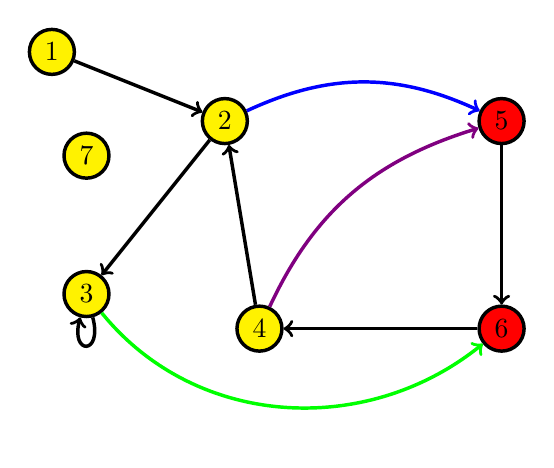
\begin{tikzpicture}
[every node/.style={inner sep=0pt}]
\node (2) [circle, minimum size=16.25pt, fill=yellow, line width=1.25pt, draw=black] at (100.0pt, -62.5pt) {\textcolor{black}{2}};
\node (4) [circle, minimum size=16.25pt, fill=yellow, line width=1.25pt, draw=black] at (112.5pt, -137.5pt) {\textcolor{black}{4}};
\node (1) [circle, minimum size=16.25pt, fill=yellow, line width=1.25pt, draw=black] at (37.5pt, -37.5pt) {\textcolor{black}{1}};
\node (5) [circle, minimum size=16.25pt, fill=red, line width=1.25pt, draw=black] at (200.0pt, -62.5pt) {\textcolor{black}{5}};
\node (6) [circle, minimum size=16.25pt, fill=red, line width=1.25pt, draw=black] at (200.0pt, -137.5pt) {\textcolor{black}{6}};
\node (3) [circle, minimum size=16.25pt, fill=yellow, line width=1.25pt, draw=black] at (50.0pt, -125.0pt) {\textcolor{black}{3}};
\node (7) [circle, minimum size=16.25pt, fill=yellow, line width=1.25pt, draw=black] at (50.0pt, -75.0pt) {\textcolor{black}{7}};
\draw [line width=1.25, ->, color=black] (1) to  (2);
\draw [line width=1.25, ->, color=black] (2) to  (3);
\draw [line width=1.25, ->, color=black, loop below] (3) to (3);
\draw [line width=1.25, ->, color=black] (6) to  (4);
\draw [line width=1.25, ->, color=black] (4) to  (2);
\draw [line width=1.25, ->, color=black] (5) to  (6);
\draw [line width=1.25, ->, color=blue] (2) to  [in=155, out=25] (5);
\draw [line width=1.25, ->, color=green] (3) to  [in=219, out=309] (6);
\draw [line width=1.25, ->, color=violet] (4) to  [in=197, out=65] (5);
\end{tikzpicture}
\end{document}
